\subsection{Distributed computing infrastructure}

% CHEP12 "Trying to Predict the Future - Resource Planning and Allocation
% in CMS" P. Kreuzer
% https://cms-mgt-conferences.web.cern.ch/cms-mgt-conferences/conferences/pres_display.aspx?cid=665&pid=4582

% CHEP10 "Experience with the CMS Computing Model from commissioning to
% collisions" D. Bonacorsi
% https://cms-mgt-conferences.web.cern.ch/cms-mgt-conferences/conferences/pres_display.aspx?cid=462&pid=2306

% CHEP10 "Monitoring the Readiness and Utilization of the Distributed CMS
% Computing Facilities during the first year LHC running" J. Hernandez
% https://cms-mgt-conferences.web.cern.ch/cms-mgt-conferences/conferences/pres_display.aspx?cid=462&pid=2332
% Note that we don't currently have monitoring in here as an explicit
% topic.  But it probably needs to be discussed in operations, at the very least.

% CHEP10 "CMS Distributed Computing Integration in the LHC sustained
% operations era" C. Grandi
% https://cms-mgt-conferences.web.cern.ch/cms-mgt-conferences/conferences/pres_display.aspx?cid=462&pid=2264

From the very start, CMS planned on having a distributed computing
infrastructure, with processing and storage resources distribued around the
world.  While HEP collaborations have historically relied on a single large
computational resource located at the host laboratory for virtually all of
their data processing and storage needs, and while a single facility would
have ultimately been more efficient to operate, it was not considered
feasible to ask the nations represented in the LHC experimental
collaborations to contribute funds for a computing center at CERN.
Instead, each nation has established domestically owned and operated sites
that contribute to the LHC experiments' computing needs.  These sites, have
given greater prominence to the LHC experiments within their participating
nations, which has led to greater funding and more engagement from local
computing experts, who would not have had a chance to participate had all
the computing been done at CERN.  CMS has successfully leveraged this local
expertise to improve the experiment's computing systems and their
operation.

The CMS distributed computing infrastructure is a tiered set of computing
sites connected through networks that follows the MONARC
model~\cite{MONARC}. The computing infrastructure is organized in a
hierarchy starting with CERN facility, called Tier 0 (T0), at its origin.
On the next level, seven regional computing centers called Tier-1 (T1)
sites form the backbone of the system, followed by Tier-2 (T2) and Tier-3
(T3) sites at universities and/or research institutes.

Sites at each tier in the hierarchy are responsible for performing certain
workflows, and the sites are configured to support those particular
workflows.  \fixme{In fact, the description of the workflows might take
  place in the ``applications'' section, we'll see, but keep some
  information here for now.}  The T0 site is responsible for data recording
and first-pass (``prompt'') data reconstruction, and also for performing
calibrations that are needed for the reconstruction.  Prompt reconstruction
starts 48 hours after events have been recorded to incorporate updated
calibrations.  The production of calibration constants is described in
Section~\ref{sec:constants}.  All events are stored in the RAW format on
tape at the T0 site.  \fixme{We'll need to be sure that RAW etc. are
  defined earlier on; this sounds like software.}  The T0 facility thus
needs substantial processing and storage resources.  At the end of Run 1,
the CMS T0 facility had \fixme{Get all the T0 parameters!}.

The primary workflows at T1 sites are the simulation of events and the
re-reconstruction of both detector and simulated events.  Simulation is a
processing-intensive workflow that requires little or no input data, but
has large output data.  Re-reconstruction of the data and simulation
samples is performed when changes to reconstruction algorithms and/or
calibrations result in reconstruction output that is sufficiently different
from that of the prompt reconstruction to have a significant impact on
understanding the physics of the LHC collisions.  The re-reconstruction
workflow also requires substantial processing resources, and both the input
and output data sizes are large.  In addition, the T1 sites are responsible
for maintaining a second archived copy of the data in RAW format, so that,
between the T0 and T1 sites, there are two tape copies of every event.  To
fulfill all of these missions, T1 sites must host processing, disk and tape
resources.  CMS operated seven T1 sites during Run 1, hosted by Germany,
Spain, France, Italy, Taiwan, the United Kingdom and the United States.  At
the end of the run, the aggregated Tier 1 resources were \fixme{Get all the
  T1 parameters!  Do we discuss relative sizes of sites?  Mention the
  hosting institutions?}

T2 sites are also responsible for some simulation workflows, and for
analysis of data and simulation samples by physics users; no user analysis
takes place at T0 or T1.  The input datasets for analysis are distributed
to the sites in advance, and then jobs seeking to analyze a particular
dataset are sent to a site that hosts the data.  While the input data for
analysis is typically large, the output is usually several orders of
magnitude smaller, as users reduce and refine the data to meet their
specific interests and needs.  \fixme{Give some typical sizes for these?
  Does such a thing exist?  Will it be elsewhere?}  T2 sites do no archival
storage, so are only required to deploy disk and processing resources.  In
Run 1, there were about fifty T2 sites, which in aggregate provided
\fixme{Get all the T2 parameters!}.  An important distinction between T2
sites and those at T0 and T1 is that the former only offer business-hour
site support and are unattended in between.

T3 sites are owned and managed by individual institutes, at a support level
of their choosing, and they execute workflows of their choosing.  T3 sites
are most often used for final-stage data analysis by the local users of the
site.  There is no set configuration for the T3 sites.

For all of the workflows, the input data must reside at the site where the
workflow is executed.  In many cases the data needs to be transferred from
another site.  All sites are interconnected via dedicated or general
purpose scientific networks. The original design separated the T2 sites
into groups that were associated with and connected to only one T1. During
LHC Run 1, the strength and reliability of the networks allowed for a more
flexible setup, realizing a full-mesh network topology where every T2 site
is connected to every T1 site and every other T2 site, as shown in
Figure~\ref{fig:distributed_topology}.  The full-mesh network allowed for
much greater ease in data movement, as a given T2 site could receive data
from a large number of potential source sites, and greater flexibility in
operations, as it was easier to move a particular dataset to a given site
so that the necessary workflows could be performed there.

\begin{figure}
\begin{center}
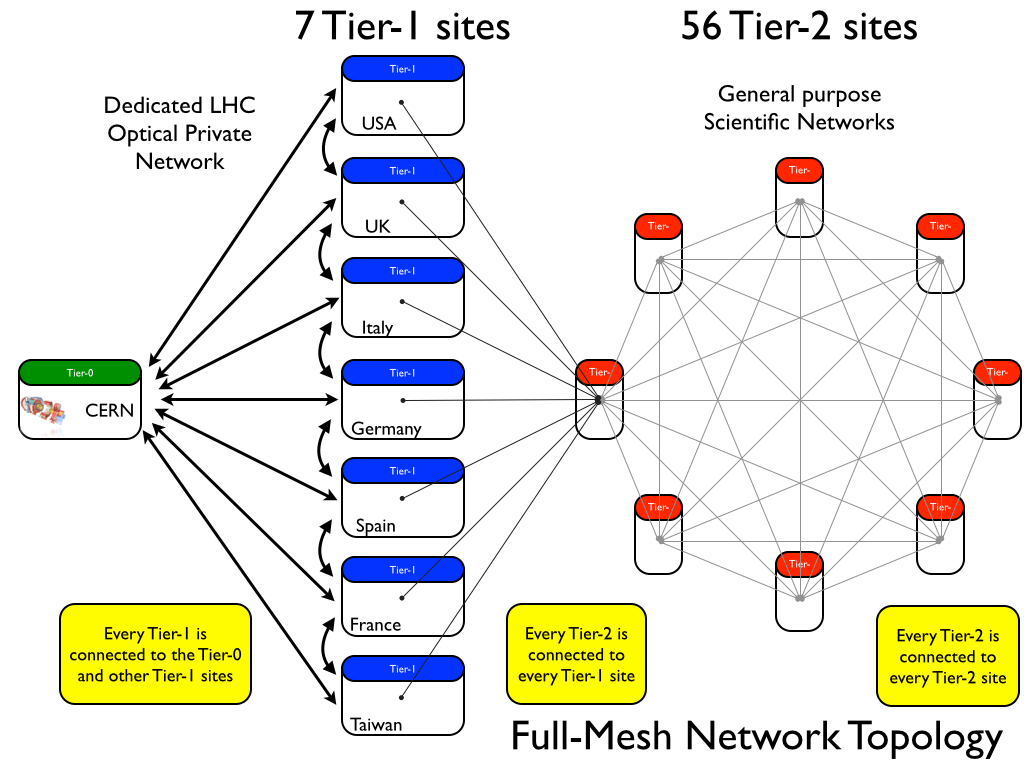
\includegraphics[width=.5\textwidth]{figs/distributed_topology}
\end{center}
\caption{The tiered CMS computing infrastructure showing the Tier-0, Tier-1 and Tier-2 levels interconnected with dedicated or general purpose scientific networks in a full-mesh network topology.
  \label{fig:distributed_topology}}
\end{figure}

The network between the sites is the backbone of the CMS computing
infrastructure, whose operation relies on transferring files among the
sites for access. The network between the T0 and T1 sites is the dedicated
LHC Optical Private Network (LHCOPN).~\fixme{Does this get a
  reference?}. The T2 sites are connected through general purpose
scientific networks in their host countries. The main data flows can be
separated into archiving and serving. Archiving is tape based where related
files are grouped by physics content on separate sets of tape cartridges
(known as tape families) to optimize writing, recall, and
recycling. Serving is disk based. The main data flows are as follows:

\begin{itemize}
\item {\bf T0 $\to$ T1}: RAW data recorded by the detector is recorded at
  T0 and stored on tape as a ``cold'' backup replica. The RAW is
  distributed across the T1's via the LHCOPN network links and archived on
  tape. The tape replica at the T1's can be recalled at any time and is
  called the custodial replica. The mass storage system at the T1's also
  provides caching capabilities and the files from the current year of data
  taking are kept cached.

\item {\bf T1 $\to$ T1}: Both RAW and simulated data are reconstructed for
  analysis on the T1 level. This requires especially strong I/O
  capabilities. The resulting AOD holds the minimum amount of information
  needed for analysis and is archived at the Tier-1 that stored the
  custodial tape copy of the input data.

\item {\bf T1 $\to$ T2}: As data of all formats is archived at T1 sites,
  which do not allow access by regular analysis users, any dataset that an
  analysis user requires must be transferred to a T2 site.  T2 disk is
  logically separated into managed portions for common samples and
  unmanaged areas for files belonging to individual users and physics
  groups.

\item {\bf T2 $\to$ T1}: The output of the simulation of a specific physics
  process at a T2 site is consolidated at a Tier-1 site where it is stored
  on tape.
\end{itemize}

An important distinction between T2 sites and those at T0 and T1 is that
the latter were used by a small number of operators for centrally-organized
production tasks.  The T2 sites were used by physicists throught the
collaboration in a ``chaotic'' mode.  Thousands of users might submit jobs
to any given site.  To maintain scalability of management, users do not
directly log in to computers at the sites, but instead submit jobs from
their local login machine through grid technologies~\cite{thegrid}.  A
computing grid is an infrastructure that allows different administrative
domains to share access to services, processors and storage with a select
set of users and groups of users. The computing clusters that are members
of a grid provide a uniform environment for user batch jobs, even if each
cluster has some unique local configuration.  As a result, any user job
can, in principle, be executed at any site on the grid with little user
customization required.  Users of the grid resources are issued credentials
that can be attached to a batch job when it is submitted to a resource;
these credentials allow for the tracking of jobs back to individual users
and thus help maintain the cybersecurity of the participating clusters.

The technology used to operate grid sites is known as ``middleware,'' as it
has a role that is somewhere between the actual hardware that operates at a
site and the software that is run by user applications.  CMS sites operated
using three different varieties of middleware.  Most sites in Europe and
Asia used the Euopean Grid Infrastructure (EGI)~\cite{EGI} middleware,
while a few sites in Northern Europe used the Advanced Resource Connector
(ARC)~\cite{ARC} middleware.  Sites in the Western Hemisphere were part of
the Open Science Grid (OSG)~\cite{OSG}.  All sites were members of the
Worldwide LHC Computing Grid (WLCG)~\cite{WLCG}, which developed a number
of common applications for the LHC experiments.  In practice, CMS developed
a number of applications that ran on top of the middleware, to make it
easier for users to access information about the data catalogue and
calibration constants that needed to be passed to the computers that
executed the jobs.  These are described in Section\fixme{Probably the
  Workflow Execution section, but need to see how this rolls out}.

This physical infrastructure of the computing sites and the wide area
network, plus the middleware infrastructure of the grid, requires a large
number of services and applications that make it useful for the CMS
workflows.  These are described in the remainder of this section.
Section~\ref{sec:corecomponents} describes the services needed for the
creation and distribution of calibration constants, data transfers, data
management, software distribution, and job submission.
Section~\ref{sec:compops} discusses the operations model for the
infrastructure, and the tools needed to monitor sites and jobs.
Section~\ref{sec:workflow} describes the management of both production and
analysis workflows.

